\section{Organizing Memory at Read Time}
\label{sec:method}

\begin{figure}[t]\centering
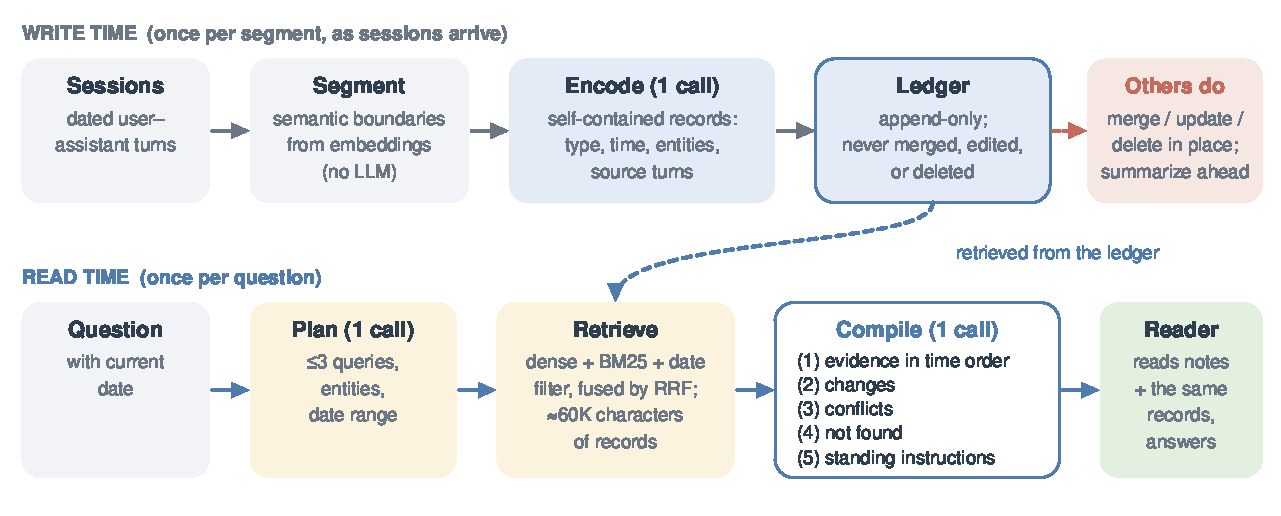
\includegraphics[width=\linewidth]{figs/fig2_method.pdf}
\caption{\textbf{\method{}.} At write time (top), each segment of a session is encoded once into self-contained,
dated records that are appended to a ledger and never merged, edited, or deleted, unlike systems that consolidate
their store in place. At read time (bottom), one call plans the search, hybrid retrieval returns about 60K characters
of records, one call compiles them into five-part evidence notes, and the reader answers from the notes and the same
records.}
\label{fig:overview}
\end{figure}

\Cref{sec:audit} suggests three requirements. The store should keep what was said without rewriting it
(\cref{sec:audit-write}); the reader should receive enough of it that retrieval is not the bottleneck
(\cref{sec:audit-loss}); and the reader should not be left to find, order, and reconcile that material on its own,
which is where Hindsight, the one long-context system in \cref{fig:loss}, loses \prelim{19.6} of its \prelim{36.3} lost points. \method{} meets them with a write side that only
appends, and a read side that retrieves broadly and then organizes what it retrieved for the question at hand
(\cref{fig:overview}). The write side and the retrieval follow LycheeMemory; what is new is the per-question compilation step and giving the reader both the notes and the records.

% M1: write side
\paragraph{Write side: an append-only ledger of atomic records.}
We follow LycheeMemory~\citep{li2026lychee} for the write side. Each session is split into segments at semantic boundaries, placed where adding the next turn would lower a segment's embedding cohesion, without an LLM. One LLM call per
segment turns it into atomic records. Each record is a self-contained statement with resolved names and absolute
dates, a type (event, fact, preference, plan, relation, or opinion), its entities and topic, the time it refers to,
and pointers to the source turns. The call also receives and updates a short disambiguation state (who is who, what
nicknames refer to, which threads are open), which carries context from one segment to the next; the state is a working variable of the encoder and is not part of the stored memory. Records are appended
and never edited, merged, or deleted: a later statement that contradicts an earlier one becomes a new record, and both
remain. A BEAM-1M conversation yields about \prelim{1,350} records.

% M2: retrieval
\paragraph{Step 1: broad retrieval.}
At question time, one short call plans the search: up to three queries, the entities the answer must involve, and a
date range if the question restricts one. Each query is run against the records twice, by dense similarity and by
BM25 over text, entities, and topic, and records inside the date range form one more ranking; reciprocal rank fusion
merges the rankings ($k=60$). We drop a record whose word-level Jaccard overlap with a higher-ranked record exceeds 0.8, attach the source turns of the six best
records, add the eight raw turns that best match the question under BM25, and fill the context up to 60K characters in rank order. This is
LycheeMemory's retrieval with a budget about eight times larger than its default; \cref{sec:audit-budget} shows that
atomic records do not lose accuracy at this budget when read directly, and \cref{sec:ablation} shows that compiling
from it is better than compiling from the default 8K.

% M3: compilation
\paragraph{Step 2: compilation into evidence notes.}
One call receives the question and the retrieved records and writes notes of at most 6,000 characters, without
answering. The notes have five parts:
(1) \emph{evidence}: every relevant item, close to the memory's own words and with its date, in time order and grouped
by thread, with names, numbers, versions, and dates kept exactly;
(2) \emph{changes}: values or plans that changed, from oldest to newest;
(3) \emph{conflicts}: statements that disagree, with both sides;
(4) \emph{not found}: the parts of the question that the memory does not cover; and
(5) \emph{standing instructions}: instructions or preferences the user gave earlier about how answers should be
written or what they should include, quoted with their date, when they could apply to this question.
Each part targets a loss we observed. Evidence in time order serves event ordering, temporal reasoning, and
summarization; changes serve knowledge updates; conflicts serve contradiction questions, where readers saw both sides
and did not raise the conflict (\cref{sec:audit-write}); ``not found'' serves abstention; and standing instructions serve instruction following: on the 10 instruction-following point questions of BEAM-100K, notes without part (5) scored \prelim{62.5}, below record retrieval with a conflict check (\prelim{70.0}), and notes with it \prelim{85.8} (three runs; \cref{sec:ablation}). Removing one part at a time (\cref{tab:noteparts}) lowers the score of the abilities each part targets with gpt-6-luna, by 1 to 2 points overall; ``not found'' has no measurable effect, and with a stronger reader no part matters. The prompt is in \cref{app:prompts}.

% M4: reader
\paragraph{Step 3: the reader reads notes and records.}
The reader receives the notes, followed by the same retrieved records, and answers with the answer prompt shared by all systems in a comparison (\cref{sec:setting}). Keeping the records serves two purposes. The notes are lossy, and the reader can check a detail against
the record it came from. And a reader that uses long contexts well can draw on material that the notes left out,
which matters for the stronger readers in \cref{sec:reader}. An earlier variant that gave the reader the notes and
only 8K characters of records needed a router to send questions about a whole topic to a larger context; giving all
questions the same input removes the router without loss (\cref{sec:ablation}).

% M5: what it costs and what it does not do
\paragraph{Cost and scope.}
At write time, \method{} makes one call per segment, about \prelim{2.3K} input and \prelim{0.8K} output tokens each.
At read time it makes three sequential calls (plan, compile, answer) with the reader model; on BEAM-1M the compilation call reads about \prelim{12K} tokens and the answer call about \prelim{15K}, fewer in total than Hindsight's single answer call over its 124K-character context (\prelim{33K}) and Hindsight\,+\,CC (\prelim{47K}; \cref{sec:cost}). Compilation is repeated for every question, so a system
that answers many questions about the same history pays it many times; caching notes across related questions is
possible but not evaluated here. \method{} does not change what is stored: errors made when a segment is encoded stay
in the ledger, and \prelim{12.0} of the \prelim{36.1} points (out of 100) that record retrieval loses on BEAM-1M come from information that no record holds (\cref{fig:loss}).
